\documentclass[journal,12pt,twocolumn]{IEEEtran}
%
\usepackage{setspace}
\usepackage{gensymb}
\usepackage{siunitx}
\usepackage{tkz-euclide} 
\usepackage{textcomp}
\usepackage{standalone}
\usetikzlibrary{calc}
\newcommand\hmmax{0}
\newcommand\bmmax{0}

%\doublespacing
\singlespacing

%\usepackage{graphicx}
%\usepackage{amssymb}
%\usepackage{relsize}
\usepackage[cmex10]{amsmath}
%\usepackage{amsthm}
%\interdisplaylinepenalty=2500
%\savesymbol{iint}
%\usepackage{txfonts}
%\restoresymbol{TXF}{iint}
%\usepackage{wasysym}
\usepackage{amsthm}
%\usepackage{iithtlc}
\usepackage{mathrsfs}
\usepackage{txfonts}
\usepackage{stfloats}
\usepackage{bm}
\usepackage{cite}
\usepackage{cases}
\usepackage{subfig}
%\usepackage{xtab}
\usepackage{longtable}
\usepackage{multirow}
%\usepackage{algorithm}
%\usepackage{algpseudocode}
\usepackage{enumitem}
\usepackage{mathtools}
\usepackage{steinmetz}
\usepackage{tikz}
\usepackage{circuitikz}
\usepackage{verbatim}
\usepackage{tfrupee}
\usepackage[breaklinks=true]{hyperref}
%\usepackage{stmaryrd}
\usepackage{tkz-euclide} % loads  TikZ and tkz-base
%\usetkzobj{all}
\usetikzlibrary{calc,math}
\usepackage{listings}
    \usepackage{color}                                            %%
    \usepackage{array}                                            %%
    \usepackage{longtable}                                        %%
    \usepackage{calc}                                             %%
    \usepackage{multirow}                                         %%
    \usepackage{hhline}                                           %%
    \usepackage{ifthen}                                           %%
  %optionally (for landscape tables embedded in another document): %%
    \usepackage{lscape}     
\usepackage{multicol}
\usepackage{chngcntr}
\usepackage{amsmath}
\usepackage{cleveref}
%\usepackage{enumerate}

%\usepackage{wasysym}
%\newcounter{MYtempeqncnt}
\DeclareMathOperator*{\Res}{Res}
%\renewcommand{\baselinestretch}{2}
\renewcommand\thesection{\arabic{section}}
\renewcommand\thesubsection{\thesection.\arabic{subsection}}
\renewcommand\thesubsubsection{\thesubsection.\arabic{subsubsection}}

\renewcommand\thesectiondis{\arabic{section}}
\renewcommand\thesubsectiondis{\thesectiondis.\arabic{subsection}}
\renewcommand\thesubsubsectiondis{\thesubsectiondis.\arabic{subsubsection}}

% correct bad hyphenation here
\hyphenation{op-tical net-works semi-conduc-tor}
\def\inputGnumericTable{}                                 %%

\lstset{
%language=C,
frame=single, 
breaklines=true,
columns=fullflexible
}
%\lstset{
%language=tex,
%frame=single, 
%breaklines=true
%}
\usepackage{graphicx}
\usepackage{pgfplots}

\begin{document}


\newtheorem{theorem}{Theorem}[section]
\newtheorem{problem}{Problem}
\newtheorem{proposition}{Proposition}[section]
\newtheorem{lemma}{Lemma}[section]
\newtheorem{corollary}[theorem]{Corollary}
\newtheorem{example}{Example}[section]
\newtheorem{definition}[problem]{Definition}
%\newtheorem{thm}{Theorem}[section] 
%\newtheorem{defn}[thm]{Definition}
%\newtheorem{algorithm}{Algorithm}[section]
%\newtheorem{cor}{Corollary}
\newcommand{\BEQA}{\begin{eqnarray}}
\newcommand{\EEQA}{\end{eqnarray}}
\newcommand{\define}{\stackrel{\triangle}{=}}
\bibliographystyle{IEEEtran}
%\bibliographystyle{ieeetr}
\providecommand{\mbf}{\mathbf}
\providecommand{\abs}[1]{\ensuremath{\left\vert#1\right\vert}}
\providecommand{\norm}[1]{\ensuremath{\left\lVert#1\right\rVert}}
\providecommand{\mean}[1]{\ensuremath{E\left[ #1 \right]}}
\providecommand{\pr}[1]{\ensuremath{\Pr\left(#1\right)}}
\providecommand{\qfunc}[1]{\ensuremath{Q\left(#1\right)}}
\providecommand{\sbrak}[1]{\ensuremath{{}\left[#1\right]}}
\providecommand{\lsbrak}[1]{\ensuremath{{}\left[#1\right.}}
\providecommand{\rsbrak}[1]{\ensuremath{{}\left.#1\right]}}
\providecommand{\brak}[1]{\ensuremath{\left(#1\right)}}
\providecommand{\lbrak}[1]{\ensuremath{\left(#1\right.}}
\providecommand{\rbrak}[1]{\ensuremath{\left.#1\right)}}
\providecommand{\cbrak}[1]{\ensuremath{\left\{#1\right\}}}
\providecommand{\lcbrak}[1]{\ensuremath{\left\{#1\right.}}
\providecommand{\rcbrak}[1]{\ensuremath{\left.#1\right\}}}
\theoremstyle{remark}
\newtheorem{rem}{Remark}
\newcommand{\sgn}{\mathop{\mathrm{sgn}}}
\providecommand{\res}[1]{\Res\displaylimits_{#1}} 
%\providecommand{\norm}[1]{\lVert#1\rVert}
\providecommand{\mtx}[1]{\mathbf{#1}}
\providecommand{\fourier}{\overset{\mathcal{F}}{ \rightleftharpoons}}
%\providecommand{\hilbert}{\overset{\mathcal{H}}{ \rightleftharpoons}}
\providecommand{\system}{\overset{\mathcal{H}}{ \longleftrightarrow}}
	%\newcommand{\solution}[2]{\textbf{Solution:}{#1}}
\newcommand{\solution}{\noindent \textbf{Solution: }}
\newcommand{\cosec}{\,\text{cosec}\,}
\providecommand{\dec}[2]{\ensuremath{\overset{#1}{\underset{#2}{\gtrless}}}}
\newcommand{\myvec}[1]{\ensuremath{\begin{pmatrix}#1\end{pmatrix}}}
\newcommand{\mydet}[1]{\ensuremath{\begin{vmatrix}#1\end{vmatrix}}}
%\numberwithin{equation}{section}
\numberwithin{equation}{subsection}
%\numberwithin{problem}{section}
%\numberwithin{definition}{section}
\makeatletter
\@addtoreset{figure}{problem}
\makeatother
\let\StandardTheFigure\thefigure
\let\vec\mathbf
%\renewcommand{\thefigure}{\theproblem.\arabic{figure}}
\renewcommand{\thefigure}{\theproblem}
%\setlist[enumerate,1]{before=\renewcommand\theequation{\theenumi.\arabic{equation}}
%\counterwithin{equation}{enumi}
%\renewcommand{\theequation}{\arabic{subsection}.\arabic{equation}}
\def\putbox#1#2#3{\makebox[0in][l]{\makebox[#1][l]{}\raisebox{\baselineskip}[0in][0in]{\raisebox{#2}[0in][0in]{#3}}}}
     \def\rightbox#1{\makebox[0in][r]{#1}}
     \def\centbox#1{\makebox[0in]{#1}}
     \def\topbox#1{\raisebox{-\baselineskip}[0in][0in]{#1}}}
\vspace{3cm}
\title{Assignment-5\\}
\author{Ayush Kumar}
\maketitle
\newpage
%\tableofcontents
\bigskip
\renewcommand{\thefigure}{\theenumi}
\renewcommand{\thetable}{\theenumi}
\begin{abstract}
This document contains solution of Problem Geolin\brak{1.12}
\end{abstract}
Download latex-tikz codes from 
%
\begin{lstlisting}
https://github.com/ayushkesh/Matrix-Theory-EE5609/tree/master/A5
\end{lstlisting}
\section{\textbf{Question}}
Find the equation of the circle that passes
through the points \myvec{2a\\0}, \myvec{0\\2b} and \myvec{a + b\\a + b}.
\section{SOLUTION}
The equation of circle can be expressed as
\begin{align}
    \vec{x}^T\vec{x}-2\vec{c}^T\vec{x}+f = 0
\end{align}
$\vec{c}$ is the centre  and substituting the points in the equation of circle we get
\begin{align}
2\myvec{2a&0}\vec{c}-f=4a^2\\
2\myvec{0&2b}\vec{c}-f=4b^2\\
2\myvec{a+b&a+b}\vec{c}-f=2\brak{a+b}^2
\end{align}
which can be expressed in matrix form
\begin{align}
\myvec{4a&0&-1\\0&4b&-1\\2\brak{a+b}&2\brak{a+b}&-1}\myvec{\vec{c}\\f} = \myvec{4a^2\\4b^2\\2\brak{a+b}^2}
\end{align}
Row reducing the augmented matrix
\begin{align}
\myvec{4a&0&-1&4a^2\\0&4b&-1&4b^2\\2\brak{a+b}&2\brak{a+b}&-1&2\brak{a+b}^2}\\
\xleftrightarrow[R_3\leftarrow R_3-2\brak{a+b}R_1]{R_1\leftarrow \frac{R_1}{4 a}}
\myvec{1 & 0 & - \frac{1}{4 a} & a \\ 0 & 4 b & -1 & 4 b^{2} \\ 0 & 2 \brak{a + b}& \frac{-a + b}{2 a} & 2b\brak{a + b}}\\
\xleftrightarrow[R_2\leftarrow \frac{R_2}{4 b}]{R_3\leftarrow R_3-2\brak{a + b}R_2}
\myvec{1 & 0 & - \frac{1}{4 a} & a \\ 0 & 1 & - \frac{1}{4 b} & b \\ 0 & 0 & \frac{a}{2 b} + \frac{b}{2 a} & 0}\\
\xleftrightarrow[]{R_3\leftarrow \frac{R_3}{\frac{a}{2b} + \frac{b}{2a}}}
\myvec{1 & 0 & - \frac{1}{4 a} & a \\ 0 & 1 & - \frac{1}{4 b} & b \\ 0 & 0 & 1 & 0}\\
\xleftrightarrow[R_1\leftarrow R_1-\brak{-\frac{1}{4 a}}R_3]{R_2\leftarrow R_2-\brak{-\frac{1}{4 b}}R_3}
\myvec{1 & 0 & 0 & a \\ 0 & 1 & 0 & b \\ 0 & 0 & 1 & 0}
\end{align}
\begin{align}
    \vec{c} = \myvec{a\\b}\\
    f = 0\\
    r=\sqrt{\norm{\vec{c}}^2-f} = \sqrt{\brak{a^2+b^2}}
\end{align}
The required equation of circle is 
\begin{align}
\vec{x}^T\vec{x}-2\myvec{a&b}\vec{x} = 0
\end{align}
\begin{figure}[!ht]
\centering
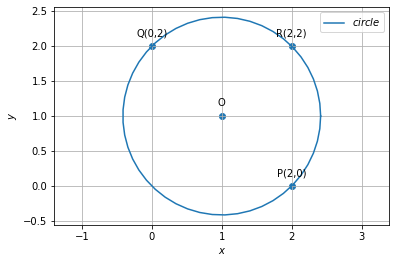
\includegraphics[width=\columnwidth]{5.png}
\caption{Circle passing through point P and Q and R}
\label{Fig:5}
\end{figure}
Python Code to verify your result, Assuming value of a=1 and b=1, 
\begin{lstlisting}
https://github.com/ayushkesh/Matrix-Theory-EE5609/tree/master/A5.py
\end{lstlisting}

\end{document}
